\begin{figure*}
    \centering
    \begin{subfigure}[b]{0.35\textwidth}
   \begin{adjustbox}{width=\linewidth}
      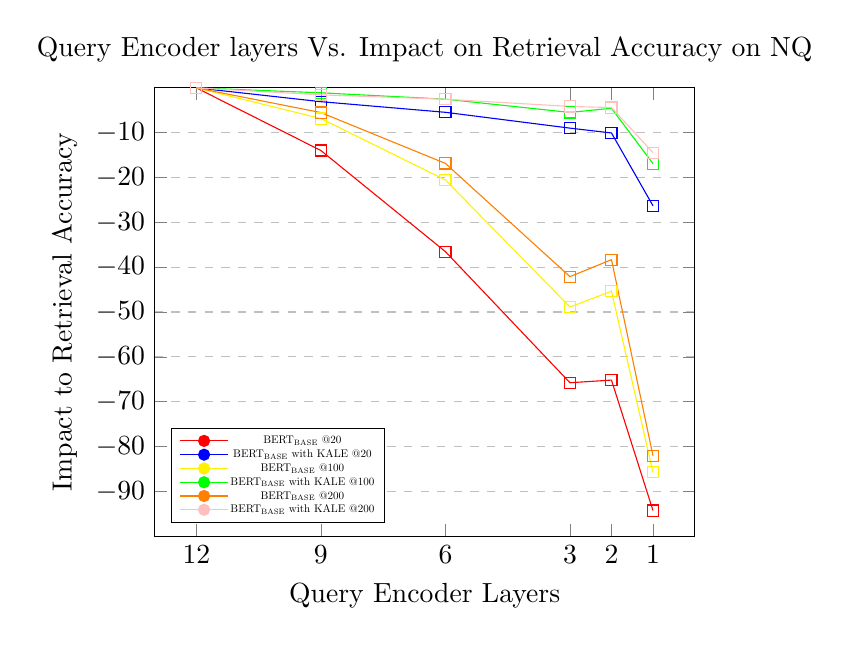
\begin{tikzpicture}
\begin{axis}[
    title={Query Encoder layers Vs. Impact on Retrieval Accuracy on NQ},
    xlabel={Query Encoder Layers},
    ylabel={Impact to Retrieval Accuracy},
    xmin=0, xmax=13,
    x dir=reverse,
    ymin=-100 , ymax=0,
    xtick={1,2,3,6,9,12},
    ytick={-10,-20,-30,-40, -50,-60,-70,-80,-90},
    legend pos=south west,
    ymajorgrids=true,
    grid style=dashed,
    legend style={nodes={scale=0.4, transform shape}}, 
    legend image post style={mark=*}
]
\addplot[
    color=red,
    mark=square,
    ]
    coordinates {
    (12, 0) (9, -13.97) (6,-36.53) (3,-65.77) (2, -65.18) (1, -94.28)
    };

\addplot[
    color=blue,
    mark=square,
    ]
    coordinates {
    (12, 0) (9, -3.08) (6, -5.45) (3,-8.98) (2,-10.06) (1, -26.30)

    };
\addplot[
    color=yellow,
    mark=square,
    ]
    coordinates {
    (12, 0) (9, -6.84) (6,-20.55) (3,-48.88) (2, -45.36) (1, -85.76)
    };

\addplot[
    color=green,
    mark=square,
    ]
    coordinates {
    (12, 0) (9, -1.10) (6, -2.52) (3,-5.48) (2,-4.54) (1, -16.90)

    };
\addplot[
    color=orange,
    mark=square,
    ]
    coordinates {
    (12, 0) (9, -5.51) (6,-16.85) (3,-42.11) (2, -38.32) (1, -82.05)
    };

\addplot[
    color=pink,
    mark=square,
    ]
    coordinates {
    (12, 0) (9, -1.56) (6, -2.53) (3,-4.14) (2,-4.39) (1, -14.44)

    };
\legend{BERT\textsubscript{BASE} @20, BERT\textsubscript{BASE} with KALE @20,BERT\textsubscript{BASE} @100, BERT\textsubscript{BASE} with KALE @100,BERT\textsubscript{BASE} @200, BERT\textsubscript{BASE} with KALE @200}
 \end{axis}
\end{tikzpicture}
 \end{adjustbox} 
\end{subfigure} 
    \begin{subfigure}[b]{0.382\textwidth}
   \begin{adjustbox}{width=\linewidth} 
      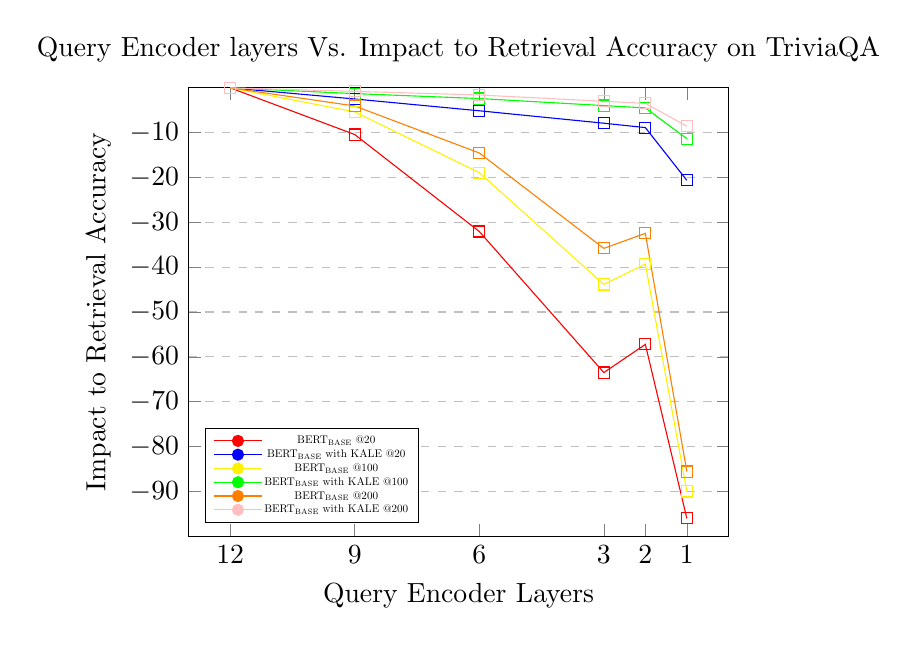
\begin{tikzpicture}
        \begin{axis}[
            title={Query Encoder layers Vs. Impact to Retrieval Accuracy on TriviaQA},
            xlabel={Query Encoder Layers},
            ylabel={Impact to Retrieval Accuracy},
            xmin=0, xmax=13,
            x dir=reverse,
            ymin=-100 , ymax=0,
            xtick={1,2,3,6,9,12},
            ytick={-10,-20,-30,-40, -50,-60,-70,-80,-90},
            legend pos=south west,
            ymajorgrids=true,
            grid style=dashed,
            legend style={nodes={scale=0.4, transform shape}}, 
            legend image post style={mark=*}
        ]
        \addplot[
            color=red,
            mark=square,
            ]
            coordinates {
            (12, 0) (9, -10.41) (6,-32.04) (3,-63.5) (2, -57.22) (1, -96.03)
            };
        
        \addplot[
            color=blue,
            mark=square,
            ]
            coordinates {
            (12, 0) (9, -2.48) (6, -5.11) (3,-7.88) (2,-8.86) (1, -20.63)
        
            };
        \addplot[
            color=yellow,
            mark=square,
            ]
            coordinates {
            (12, 0) (9, -5.35) (6,-18.91) (3,-43.84) (2, -39.29) (1, -90.02)
            };
        
        \addplot[
            color=green,
            mark=square,
            ]
            coordinates {
            (12, 0) (9, -1.28) (6,-2.38) (3,-3.95) (2, -4.47) (1, -11.33)
            };
        
        \addplot[
            color=orange,
            mark=square,
            ]
            coordinates {
            (12, 0) (9, -4.04) (6, -14.52) (3,-35.8) (2,-32.45) (1, -85.58)
        
            };
        \addplot[
            color=pink,
            mark=square,
            ]
            coordinates {
            (12, 0) (9, -0.78) (6,-1.59) (3,-2.99) (2, -3.45) (1, -8.54)
            };
        \legend{BERT\textsubscript{BASE} @20, BERT\textsubscript{BASE} with KALE @20,BERT\textsubscript{BASE} @100, BERT\textsubscript{BASE} with KALE @100,BERT\textsubscript{BASE} @200, BERT\textsubscript{BASE} with KALE @200}
         \end{axis}
        \end{tikzpicture}
         \end{adjustbox}       
    \end{subfigure}
    \\
    \begin{subfigure}[b]{0.4\textwidth}
       \begin{adjustbox}{width=\linewidth} % rescale box
          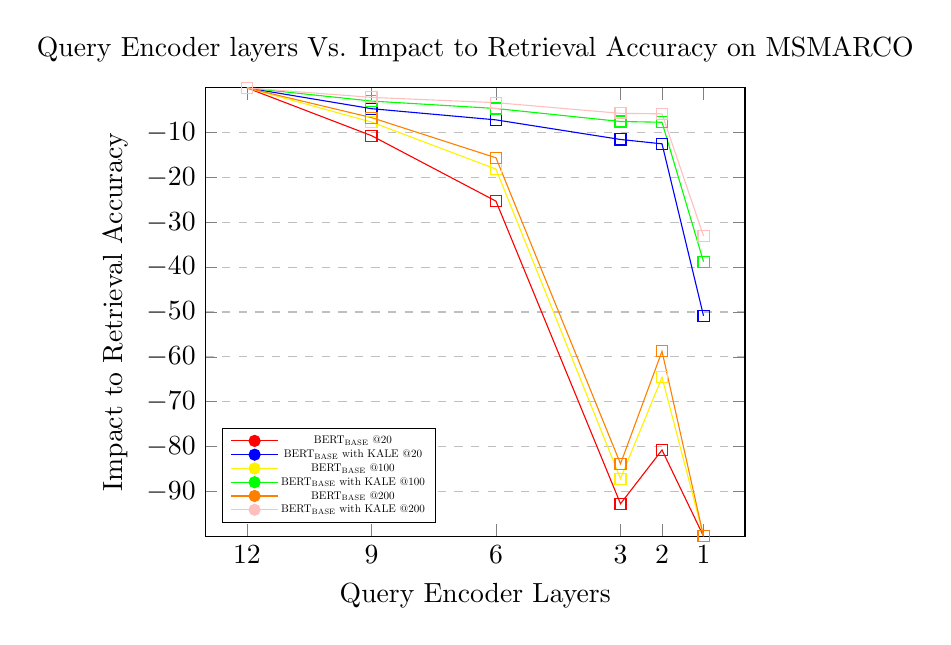
\begin{tikzpicture}
            \begin{axis}[
                title={Query Encoder layers Vs. Impact to Retrieval Accuracy on MSMARCO},
                xlabel={Query Encoder Layers},
                ylabel={Impact to Retrieval Accuracy},
                xmin=0, xmax=13,
                x dir=reverse,
                ymin=-100 , ymax=0,
                xtick={1,2,3,6,9,12},
                ytick={-10,-20,-30,-40, -50,-60,-70,-80,-90},
                legend pos=south west,
                ymajorgrids=true,
                grid style=dashed,
                legend style={nodes={scale=0.4, transform shape}}, 
                legend image post style={mark=*}
            ]
            \addplot[
                color=red,
                mark=square,
                ]
                coordinates {
                (12, 0) (9, -10.65) (6,-25.27) (3,-92.76) (2, -80.77) (1, -100)
                };
            
            \addplot[
                color=blue,
                mark=square,
                ]
                coordinates {
                (12, 0) (9, -4.64) (6, -7.14) (3,-11.51) (2,-12.48) (1, -50.84)
            
                };
            \addplot[
                color=yellow,
                mark=square,
                ]
                coordinates {
                (12, 0) (9, -7.62) (6,-18.12) (3,-87.17) (2, -64.56) (1, -100)
                };
            
            \addplot[
                color=green,
                mark=square,
                ]
                coordinates {
                (12, 0) (9, -2.94) (6, -4.6) (3,-7.5) (2,-7.67) (1, -38.77)
            
                };
            \addplot[
                color=orange,
                mark=square,
                ]
                coordinates {
                (12, 0) (9, -6.63) (6,-15.6) (3,-83.85) (2, -58.75) (1, -100)
                };
            
            \addplot[
                color=pink,
                mark=square,
                ]
                coordinates {
                (12, 0) (9, -2.12) (6, -3.3) (3,-5.68) (2,-5.79) (1, -33.05)
            
                };
            \legend{BERT\textsubscript{BASE} @20, BERT\textsubscript{BASE} with KALE @20,BERT\textsubscript{BASE} @100, BERT\textsubscript{BASE} with KALE @100,BERT\textsubscript{BASE} @200, BERT\textsubscript{BASE} with KALE @200}
             \end{axis}
            \end{tikzpicture}
        \end{adjustbox}       
    \end{subfigure} \\ 
    \begin{subfigure}[b]{0.38\textwidth}
       \begin{adjustbox}{width=\linewidth} % rescale box
          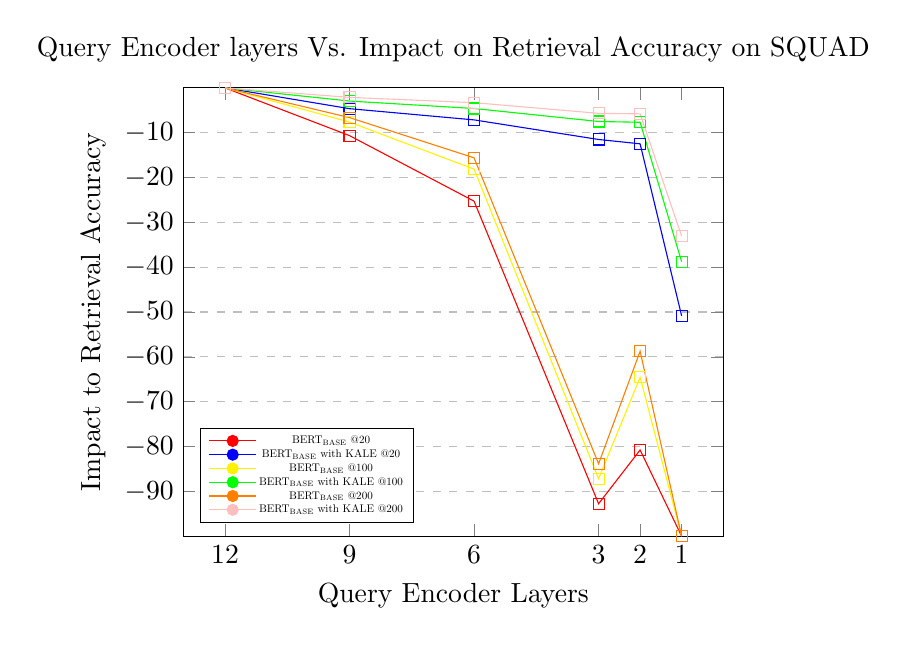
\begin{tikzpicture}
            \begin{axis}[
                title={Query Encoder layers Vs. Impact on Retrieval Accuracy on SQUAD},
                xlabel={Query Encoder Layers},
                ylabel={Impact to Retrieval Accuracy},
                xmin=0, xmax=13,
                x dir=reverse,
                ymin=-100 , ymax=0,
                xtick={1,2,3,6,9,12},
                ytick={-10,-20,-30,-40, -50,-60,-70,-80,-90},
                legend pos=south west,
                ymajorgrids=true,
                grid style=dashed,
                legend style={nodes={scale=0.4, transform shape}}, 
                legend image post style={mark=*}
            ]
            \addplot[
                color=red,
                mark=square,
                ]
                coordinates {
                (12, 0) (9, -10.65) (6,-25.27) (3,-92.76) (2, -80.77) (1, -100)
                };
            
            \addplot[
                color=blue,
                mark=square,
                ]
                coordinates {
                (12, 0) (9, -4.64) (6, -7.14) (3,-11.51) (2,-12.48) (1, -50.84)
            
                };
            \addplot[
                color=yellow,
                mark=square,
                ]
                coordinates {
                (12, 0) (9, -7.62) (6,-18.12) (3,-87.17) (2, -64.56) (1, -100)
                };
            
            \addplot[
                color=green,
                mark=square,
                ]
                coordinates {
                (12, 0) (9, -2.94) (6, -4.6) (3,-7.5) (2,-7.67) (1, -38.77)
            
                };
            \addplot[
                color=orange,
                mark=square,
                ]
                coordinates {
                (12, 0) (9, -6.63) (6,-15.6) (3,-83.85) (2, -58.75) (1, -100)
                };
            
            \addplot[
                color=pink,
                mark=square,
                ]
                coordinates {
                (12, 0) (9, -2.12) (6, -3.3) (3,-5.68) (2,-5.79) (1, -33.05)
            
                };
            \legend{BERT\textsubscript{BASE} @20, BERT\textsubscript{BASE} with KALE @20,BERT\textsubscript{BASE} @100, BERT\textsubscript{BASE} with KALE @100,BERT\textsubscript{BASE} @200, BERT\textsubscript{BASE} with KALE @200}
             \end{axis}
            \end{tikzpicture}
        \end{adjustbox}
    \end{subfigure} 
    \begin{subfigure}[b]{0.4\textwidth}
       \begin{adjustbox}{width=\linewidth} % rescale box
          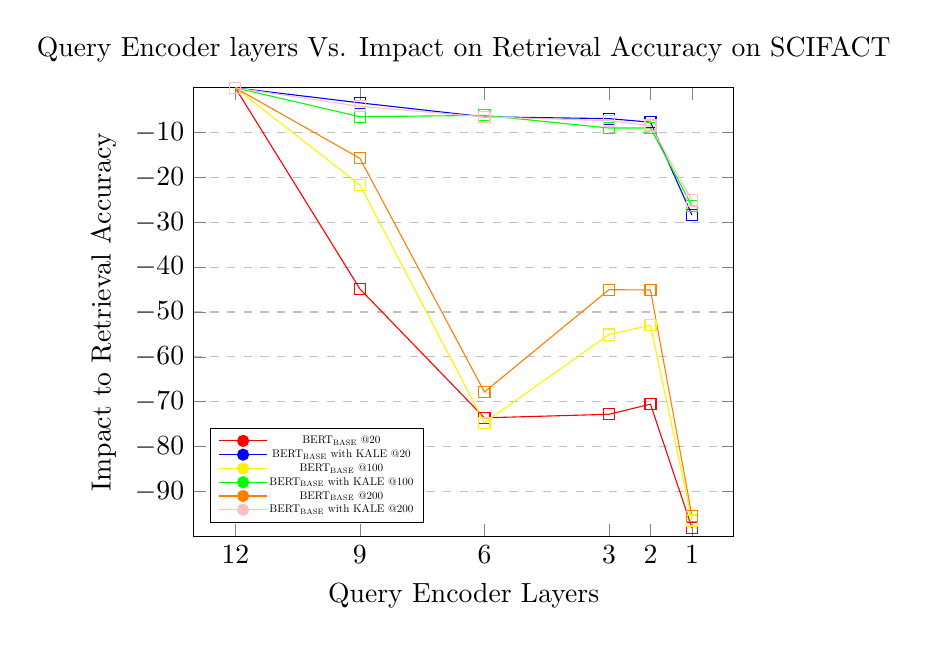
\begin{tikzpicture}
            \begin{axis}[
                title={Query Encoder layers Vs. Impact on Retrieval Accuracy on SCIFACT},
                xlabel={Query Encoder Layers},
                ylabel={Impact to Retrieval Accuracy},
                xmin=0, xmax=13,
                x dir=reverse,
                ymin=-100 , ymax=0,
                xtick={1,2,3,6,9,12},
                ytick={-10,-20,-30,-40, -50,-60,-70,-80,-90},
                legend pos=south west,
                ymajorgrids=true,
                grid style=dashed,
                legend style={nodes={scale=0.4, transform shape}}, 
                legend image post style={mark=*}
            ]
            \addplot[
                color=red,
                mark=square,
                ]
                coordinates {
                (12, 0) (9, -44.85) (6,-73.60) (3,-72.81) (2, -70.55) (1, -98.18)
                };
            
            \addplot[
                color=blue,
                mark=square,
                ]
                coordinates {
                (12, 0) (9, -3.34) (6,-6.45) (3,-6.86) (2, -7.66) (1, -28.38)
                };
            \addplot[
                color=yellow,
                mark=square,
                ]
                coordinates {
                (12, 0) (9, -21.64) (6,-74.66) (3,-55.02) (2, -52.95) (1, -96.50)
                };
            
            \addplot[
                color=green,
                mark=square,
                ]
                coordinates {
                (12, 0) (9, -6.43) (6,-6.14) (3,-8.96) (2, -8.96) (1, -26.32)
                };
            \addplot[
                color=orange,
                mark=square,
                ]
                coordinates {
                (12, 0) (9, -15.72) (6,-67.83) (3,-45.01) (2, -45.09) (1, -95.49)
                };
            
            \addplot[
                color=pink,
                mark=square,
                ]
                coordinates {
                (12, 0) (9, -4.13) (6,-6.47) (3,-7.33) (2, -8.39) (1, -25.11)
                };
            \legend{BERT\textsubscript{BASE} @20, BERT\textsubscript{BASE} with KALE @20,BERT\textsubscript{BASE} @100, BERT\textsubscript{BASE} with KALE @100,BERT\textsubscript{BASE} @200, BERT\textsubscript{BASE} with KALE @200}
             \end{axis}
            \end{tikzpicture}
        \end{adjustbox}
    \end{subfigure}
    \caption{Impact of structural pruning with and without KALE on the NQ, MSMARCO, TriviaQA, SciFACT, and SQuAD Passage Retrieval dataset with the recall set sizes of 20,100, and 200. Across datasets, we see a consistent trend where KALE is effective but most effective when the network is heavily pruned and recall set sizes are small. When the model is pruned to 2 or 1 layer with a recall set size of 20, the difference between using KALE or not can be up to 10 times the loss in recall accuracy}
    \label{fig:kale-not}
\end{figure*}